\documentclass{beamer}
\usepackage{default}
\usepackage{amsthm}
\usepackage{graphicx}
\begin{document}
\begin{frame}{Boolean Operation}

Some operations of ordinary algebra, in particular,multiplication xy, 
addition x + y, and negation −x, have their counterparts in Boolean algebra.
Those operations are :- 

\begin{itemize}
  \item \textbf{\underline{AND}}
  \item \textbf{\underline{OR}}
  \item \textbf{\underline{NOT}}
\end{itemize}
\end{frame}

\begin{frame}{Basic Boolean operators}
\begin{itemize}
 \item AND - It's symbol is “∧” and  it is used as multiplication counterpart of linear algebra.
	     It is called conjunction in boolean language.
 \item OR -  It's symbol is “∨” and  it is used as addition counterpart of linear algebra.
	     It is called disjunction in boolean language.
 \item NOT - Its symbol is “¬” and “!”and it is used as negation counterpart of linear algebra.
	     It is called negation or complement in boolean language.
\end{itemize}
\end{frame}

\begin{frame}{AND operator}
\begin{figure}
\centering
\caption{ The distinctive shape of AND gate}
\label{and:and}
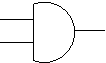
\includegraphics{and}
\end{figure}


  The AND gate is a basic digital logic gate that implements logical conjunction. 
  A HIGH output(1) results only if both the inputs to the AND gate are HIGH (1). 
  If neither or only one input to the AND gate is HIGH, a LOW output results.

  \begin{table}
   \centering
   \begin{tabular}{|l c r|}
      input in A	&input in B	&output(A AND B) \\
      0			&0		&0		\\
      0			&1		&0		\\
      1			&0		&0		\\
      1			&1		&1
   \end{tabular}
\caption{showing the result of AND operator for different values of A and B}
   \end{table}
  
\end{frame}

\begin{frame}{OR operator}

\begin{figure}
\centering
\caption{ The distinctive shape of OR gate}
\label{or:or}
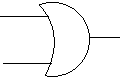
\includegraphics{or}
\end{figure}
 The OR gate is a digital logic gate that implements logical disjunction.
 A HIGH output (1) results if one or both the inputs to the gate are HIGH (1). 
 If neither input is HIGH, a LOW output (0) results.
  \begin{table}
   \centering
   \begin{tabular}{|l c r|}
      input in A	&input in B	&output(A AND B) \\
      0			&0		&0		\\
      0			&1		&1		\\
      1			&0		&1		\\
      1			&1		&1
   \end{tabular}
\caption{showing the result of OR operator for different values of A and B}
   \end{table}
\end{frame}

\begin{frame}{NOT operator}
\begin{figure}
\centering
\caption{ The distinctive shape of NOT gate}
\label{not:not}
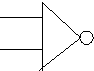
\includegraphics{not}
\end{figure}

A NOT gate is a logic gate which implements logical negation. 
\begin{table}
   \centering
   \begin{tabular}{|l c|}
      input in A	&output in A \\
      0			&1		\\
      1			&0		\\
 
   \end{tabular}
\caption{showing the result of OR operator for different values of A and B}
   \end{table}

   \end{frame}

   
\begin{frame}{De Morgan's Laws in Boolean Algebra}

\newtheorem{first}{First Law}
\begin{first}
The negation of a conjunction is the disjunction of the negations. \\
\end{first}

\newtheorem{second}{Second Law}
\begin{second}
The negation of a disjunction is the conjunction of the negations. \\ 
\end{second}

The two laws can be stated in mathematical statement or boolean language for two boolean values P and Q as :-

    $\neg(P\land Q)\iff(\neg P)\lor(\neg Q)$
    \\
    $\neg(P\lor Q)\iff(\neg P)\land(\neg Q)$

\end{frame}

\begin{frame}{First Law}

\textbf{\underline{The negation of a conjunction is the disjunction of the negations}}. \\
\begin{proof}
\begin{table}
\centering
\begin{tabular}{|r r r r r r r|}

P 	&Q 	&$P \land Q$ 	&$\neg(P \land Q)$ 	&$\neg P$ 	&$\neg Q$ 	&$\neg(P)\lor \neg(Q)$ \\
0 	&0 	&0 		&1 			&1 		&1 		&1 \\
0 	&1 	&1		&0 			&1 		&0 		&0 \\ 
1 	&0 	&1 		&0 			&0 		&1 		&0 \\
1 	&1 	&1 		&0 			&0 		&0 		&0

\end{tabular}
\end{table}
From the table, it can be easily seen that
    $\neg(P\land Q)\iff(\neg P)\lor(\neg Q)$

\end{proof}
\end{frame}

\begin{frame}{Second Law}

\textbf{\underline{The negation of a disjunction is the conjunction of the negations}}. \\
\begin{proof}
\begin{table}
\centering
\begin{tabular}{|r r r r r r r|}

p 	&q 	&$p \lor q$ 	&$\neg(p \lor q)$ 	&$\neg p$ 	&$\neg q$ 	&$(\neg p)\land(\neg q)$ \\
0 	&0 	&0 		&1 			&1 		&1 		&1 \\
0 	&1 	&0		&1 			&1 		&0 		&1 \\ 
1 	&0 	&0 		&1 			&0 		&1 		&1 \\
1 	&1 	&1 		&0 			&0 		&0 		&0

\end{tabular}
\end{table}
From the table, it can be easily seen that
$\neg(P\lor Q)\iff(\neg P)\land(\neg Q)$

\end{proof}
\end{frame}

\begin{frame}{De Morgan's laws for n variables $A_i$}
For n variables ,De Morgan's laws are genrally written as:
\\
    $\overline{\bigcap_{i \in I} A_{i}}\equiv \bigcup_{i \in I} \overline{A_{i}}$ \\

    $\overline{\bigcup_{i \in I} A_{i}}\equiv 	\bigcap_{i \in I} \overline{A_{i}}$
\\
where I is the set of n variables $A_i$
\end{frame}


\end{document}
